% FRC 控制工程 —— 中文译本
% 原著：Controls Engineering in the FIRST Robotics Competition (Tyler Veness)
% 原著采用 CC BY-SA 4.0 许可；本译本仅供学习交流
% 编译：xelatex main.tex （运行两遍以生成目录与交叉引用）
\documentclass[UTF8,a4paper,zihuan=-4,fontset=windows,openany]{ctexbook}

\usepackage[margin=2.5cm]{geometry}
\usepackage{amsmath,amssymb,amsthm}
\usepackage{graphicx}
\usepackage{booktabs}
\usepackage[most]{tcolorbox}
\usepackage{enumitem}
\usepackage{caption}
\usepackage[colorlinks=true,linkcolor=blue!50!black,urlcolor=blue!60!black,citecolor=blue!50!black]{hyperref}

\graphicspath{{figures/}}
\captionsetup{font=small}
\allowdisplaybreaks
\setcounter{tocdepth}{1}

% 三重/四重牛顿记号（加点）
\newcommand{\dottriple}[1]{\overset{\cdot\cdot\cdot}{#1}}
\newcommand{\dotquad}[1]{\overset{\cdot\cdot\cdot\cdot}{#1}}

% 译注/提醒框（原著中的 "R" 标记）
\newtcolorbox{tip}[1][注]{enhanced,breakable,
  colback=orange!8,colframe=orange!85!black,boxrule=0.8pt,arc=1.5mm,
  left=2mm,right=2mm,top=1.5mm,bottom=1.5mm,title={#1},fonttitle=\bfseries}

% 视频等外部资源框
\newtcolorbox{media}[1][扩展资源]{enhanced,breakable,
  colback=blue!6,colframe=blue!65!black,boxrule=0.8pt,arc=1.5mm,
  left=2mm,right=2mm,top=1.5mm,bottom=1.5mm,title={#1},fonttitle=\bfseries}

% 章首照片（原著各章开头的风景照）。用法：\chapterphoto{照片说明}{文件名}
\newcommand{\chapterphoto}[2]{%
  \clearpage
  \thispagestyle{plain}%
  \noindent
  \begin{minipage}{\textwidth}\centering
    \includegraphics[height=4.2cm,keepaspectratio]{#2}\\[3pt]
    {\footnotesize\color{gray!60} #1}
  \end{minipage}\par}

% 定义环境（定义 2.1.1 —— 名称）
\newtheoremstyle{cnplain}
  {\topsep}{\topsep}{}{}{\bfseries}{.}{.5em}{}
\theoremstyle{cnplain}
\newtheorem{definition}{定义}[section]

\title{\Huge FRC 控制工程\\[0.8em]
  \large Controls Engineering in the FIRST Robotics Competition\\[0.5em]
  \normalsize 中文译本（第一部分：控制理论基础）}
\author{Tyler Veness 著}
\date{}

\begin{document}

\frontmatter
\maketitle
\tableofcontents

\chapterphoto{加利福尼亚州圣玛丽亚 Spencer 市场附近的花丛}{photo-preface}
\chapter*{前言}
\addcontentsline{toc}{chapter}{前言}

当我还是 FIRST 机器人竞赛（FRC）3512 队的一名高中生时，我只能从互联网上零散的资料中学习控制理论——这些资料要么不够严谨，要么预设了过多的先验知识。后来我在加州大学圣克鲁兹分校（UCSC）攻读学士学位期间修读了研究生级别的控制理论课程，才意识到：只要讲述得当，这些概念其实并不难，只是这些知识在学术界之外并不容易获取。

我想弥合这种信息鸿沟，让更多的人能够领略我在控制理论中所看到的美与优雅。本书正是为了简化学习过程、使之成为可能而写的。

本书的初稿是我在 UCSC 2017 年春季一门本科技术写作课（CMPE 185）的期末项目。它最初是一篇 13 页的 IEEE 格式论文，定位为状态空间控制的参考手册和入门指南，总结了我那一年修读的三门研究生控制课程。接下来的一年里我继续充实它的内容，它最终长得足以成为一本真正的书。从那时起，随着我学到新的东西，我便不断地把它补充进本书。

我把这些内容放在 FRC 的背景之下，因为它一直是我生活中的重要组成部分，也是一个很有用的应用沙盒。后来，我把本书中许多工具的实现贡献给了 FRC 标准库（WPILib），并由我负责维护。

\section*{致谢}

感谢我的控制工程课程老师 Dejan Milutinovi\'c 和 Gabriel Elkaim，是他们将我领进了控制理论领域的大门。他们教会了我成为一名控制工程师意味着什么，我也非常欣赏他们课程中那种注重直觉与应用的务实视角。


\mainmatter
\setcounter{chapter}{-1} % 原著从第 0 章开始编号
\chapterphoto{UCSC Baskin 工程楼旁的树木}{photo-chap0}
\chapter{致读者}

\section{预备知识}
本书假定读者具备基本的代数与复数知识。必要的入门物理与微积分知识会在需要时予以讲授。

\section{本书的结构}
\label{sec:structure}
本书由五个部分和一组附录组成，涵盖控制工程师所要完成的四项任务：推导系统的模型（运动学）、为模型设计控制器（控制理论）、设计观测器来估计模型的当前状态（定位），以及规划控制器如何驱动模型到达期望状态（运动规划）。

第一部分``控制理论基础''介绍控制理论的基础知识，讲授 PID 控制器设计的基本原理。

第二部分``现代控制理论''首先以速成课的形式介绍线性代数背后的几何直觉，并讲授足够多的矩阵代数运算方法，使读者能够跟上后续章节的内容。它介绍状态空间表示、能控性与能观性。第一部分获得的直觉与线性代数的记号将被用于对线性多输入多输出（MIMO）系统进行建模和控制，内容涵盖离散化、LQR 控制器设计、LQE 观测器设计和前馈。随后，这些概念被应用于实际系统的控制器设计与实现。第四部分的例子会被转换为状态空间表示，加以实现，并用离散控制器进行测试。

第二部分还介绍了利用李雅普诺夫函数进行非线性控制系统分析的基础知识。它给出了一个独轮车（unicycle）型车辆非线性控制器的例子，以及如何将其应用于两轮车辆。由于非线性控制并不是本书的重点，我们会列出其他书籍和资源供进一步阅读。

第三部分``估计与定位''介绍随机控制理论领域。本书讲授 Luenberger 观测器以及卡尔曼滤波背后的概率论，并给出若干卡尔曼滤波理论创造性应用的例子。

第四部分``系统建模''介绍推导前述章节模型所需的基本微积分和物理概念，并逐步推导若干常见 FRC 子系统的模型。然后讨论系统辨识方法，用于通过实验测量模型参数。

第五部分``运动规划''讨论如何规划机器人从当前状态到达某个期望状态的路径，使运动在其动力学可达的范围内。它介绍用于简单机动的一自由度运动速度曲线（motion profile）。对于自由度更高的曲线，则介绍轨迹优化方法来生成。

附录提供了进一步提高的内容，并非理解本书主体所必需。其中包括对正文中所给出并使用的许多结论的推导。

案例研究中用于生成图像的 Python 脚本，同时也是相应章节所讨论技术的参考实现。它们可以在本书的 Git 仓库中找到，仓库位置见版权页。

\section{本书的理念}
\label{sec:ethos}
本书既可以作为新学生的教程，也可以作为需要温习某些内容的更有经验的读者的参考手册。虽然本书并不追求面面俱到，但希望读者读完之后能够学有所成：要么能亲自实现书中介绍的概念，要么知道去哪里查找更多信息。

书中的某些部分在数学上是严谨的，但我相信，应当让学生打下扎实的理论基础，同时侧重直觉，这样他们才能把所学应用到新的问题上。要深入理解本书的主题，数学是不可避免的。话虽如此，我仍会尽可能提供实用、直观的解释。

大多数教学资源都把线性控制和非线性控制分开讲授，后者通常留给另一门课程。在这里，我们把它们放在一起介绍，因为非线性控制的概念经常出现，而且（如果不考虑李雅普诺夫稳定性的话）这个跨越并不算大。控制与估计各章会在适当的时候介绍处理非线性的相关工具，例如线性化。

\section{无私工程师的心态}
\label{sec:mindset}
工程不只是一套技能，更是一种心态。工程师有一种独特的问题处理方式。下面的格言概括了我希望传授给我的机器人学生们的东西（例子取自控制工程领域）。

\begin{quote}
\itshape ``基于需求做工程设计，而不是基于某种意识形态。''
\end{quote}

工程充满了权衡。工具应当适配任务，并非每个问题都是等着被锤子敲的钉子。正确的做法是：评估解决当前任务所需的最低要求（最低规格），然后只做刚好能满足它们的工作；超出规格就是浪费时间和金钱。如果你需要高于最低规格的性能或可维护性，那么按定义，你的最低规格就选错了。

控制工程在类似的意义上也是务实的：解决。眼前。的问题。对于非线性系统的控制，被控对象求逆（plant inversion）在纸面上很优雅，但在模型不准确时并不奏效；而使用理论上``不正确''的解——比如对非线性系统做线性近似——效果却足够好，以至于整个工业界都在使用它。有比 PID 更复杂的控制器，但我们仍然使用 PID，就是因为它通用而简单。有时，``较差''的解反而比控制系统设计者心目中理想或``干净''的方案更有效，或者具有更划算的收益成本比。请选择最有效的工具。

解决方案只需要足够好，而不必完美。我们想避开积分器，因为它们会引入不稳定，但我们仍然使用它们，因为它们能很好地满足跟踪指标。不应盲目地捍卫某个设计或遵循某种教条，因为总存在其对立面才是更优选择的情形。工程师应当能够判断何时属于这种情况，放下自我，去做能满足客户要求的事情（例如系统响应特性、可维护性、易用性）。出于务实或技术上的原因而偏好某个方案是没有问题的，但工程师不应在个人情感上纠结于最终选择了哪个``足够好''的方案。

\section{征求反馈}
\label{sec:feedback}
虽然我们努力写出一本让控制理论变得平易近人的书，但对某些读者而言，它可能仍然显得内容密集或节奏偏快（这本薄书涵盖了三门反馈控制课程的内容，其中两门是研究生课程）。请通过版权页上列出的 GitHub 链接向我们发送反馈、勘误或建议。也欢迎提供能够展示关键概念、并使它们更易于理解的新例子。


\part{控制理论基础}
\chapterphoto{圣玛丽亚市 Rice Ranch 路旁步道附近的公路}{photo-chap1}
\chapter{控制系统基础}

控制系统无处不在，我们每天都在与它们打交道。你可能见过的一小部分例子包括：带恒温器的暖气与空调、汽车上的巡航控制和防抱死制动系统（ABS）、以及现代笔记本电脑上的风扇转速调节。控制系统监测或控制这类系统的行为；它们可以由人直接控制（手动控制），也可以完全由机器构成（自动控制）。

例如，我们如何证明自动驾驶汽车上的闭环控制器在存在不确定性的情况下仍能安全运行，并满足期望的性能指标？控制理论是代数与几何的一种应用，用来分析和预测系统的行为、让系统按我们的意愿响应，并使系统对扰动和不确定性具有鲁棒性。

简而言之，控制工程（controls engineering）就是将工程流程应用于控制理论。因此，它不仅仅是应用数学。尽管控制理论背后有一些漂亮的数学，但控制工程和其他工程学科一样，充满了权衡。对于控制理论给出的解，我们总是应当进行合理性检验，并以我们的性能指标为依据。我们不需要完美；我们只需要足够好，能够满足指标即可。\textsuperscript{[1]}

\begin{tip}
大多数高级工程主题的资料所假设的知识水平都远高于实际所需。部分原因在于行话（jargon）的使用。行话固然能在领域内高效地交流思想，但不熟悉它的新人却会一头雾水。因此，在使用术语之前先给出定义非常重要。书末的术语表列出了控制理论中的常用词汇和短语、它们的来源及其含义。书中某些词语附有指向术语表的链接，并以这种颜色显示。
\end{tip}

\section{增益是什么？}
\label{sec:gain}
增益（gain）是一个比例值，它描述稳态下输出信号幅值与输入信号幅值之间的关系。许多系统都包含可以改变增益的机制，从而能够为系统提供或多或少的``动力''。

图~\ref{fig:gain} 展示了一个具有假想输入和输出的系统。由于输出的幅值是输入的两倍，该系统的增益为 2。

\begin{figure}[htbp]
  \centering
  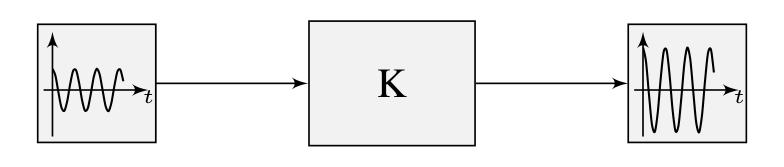
\includegraphics[width=0.75\textwidth]{fig1-1.png}
  \caption{演示增益为 $K = 2$ 的系统}
  \label{fig:gain}
\end{figure}

\section{框图}
\label{sec:blockdiagrams}
在设计或分析控制系统时，用图形来为系统建模往往很有用。框图（block diagram）正是为此目的而使用的工具。它可以被系统地操作和化简（见附录 A）。图~\ref{fig:blockdiag} 就是一个例子。

\begin{figure}[htbp]
  \centering
  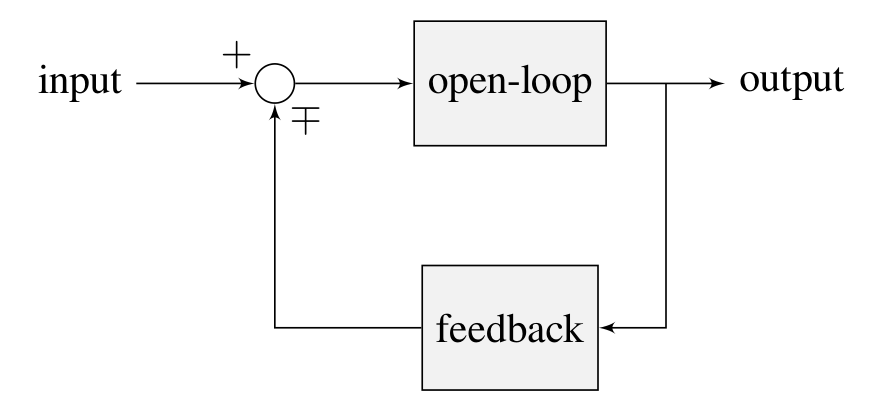
\includegraphics[width=0.7\textwidth]{fig1-2.png}
  \caption{框图及其各部分的名称}
  \label{fig:blockdiag}
\end{figure}

开环增益（open-loop gain）是从输入端的求和节点（圆圈）到输出支路的总增益。如果断开反馈回路，它就是系统的增益。

反馈增益（feedback gain）是从输出返回到输入求和节点的总增益。求和节点的输出等于其输入之和。

图~\ref{fig:feedbackdiag} 是一个采用更正式记号的反馈结构框图。

\begin{figure}[htbp]
  \centering
  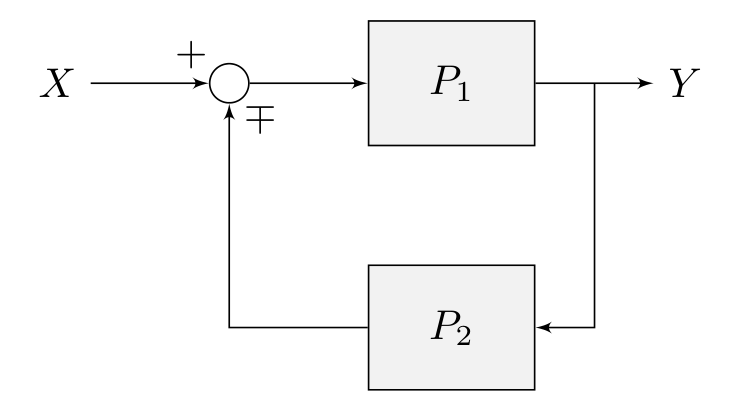
\includegraphics[width=0.45\textwidth]{fig1-3.png}
  \caption{反馈框图}
  \label{fig:feedbackdiag}
\end{figure}

$\mp$ 表示``负或正''，其中负号代表负反馈。

\section{开环系统与闭环系统}
\label{sec:openloop}
被控制系统所控制的系统或执行器的集合称为被控对象（plant）。控制器（controller）用于驱动被控对象从当前状态到达某个期望的状态（即参考值，reference）。在框图中，我们对相关量使用如下记号：

\begin{center}
\begin{tabular}{ll}
  $r(t)$ & 参考值 \\
  $u(t)$ & 控制输入 \\
  $e(t)$ & 误差 \\
  $y(t)$ & 输出 \\
\end{tabular}
\end{center}

不利用从被控对象输出处测量到的信息的控制器称为\textbf{开环控制器}或\textbf{前馈控制器}。图~\ref{fig:openloop} 展示了一个带前馈控制器的被控对象。

\begin{figure}[htbp]
  \centering
  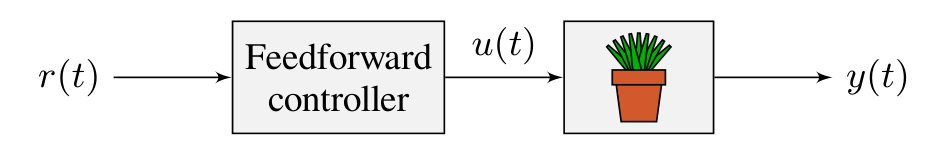
\includegraphics[width=0.8\textwidth]{fig1-4.png}
  \caption{开环控制系统}
  \label{fig:openloop}
\end{figure}

利用从被控对象输出反馈回来的信息的控制器称为\textbf{闭环控制器}或\textbf{反馈控制器}。图~\ref{fig:closedloop} 展示了一个带反馈控制器的被控对象。

\begin{figure}[htbp]
  \centering
  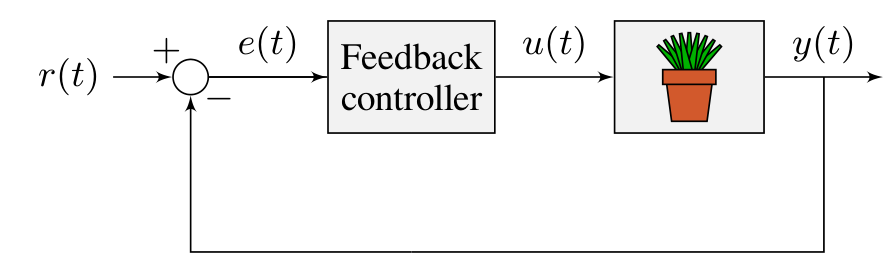
\includegraphics[width=0.7\textwidth]{fig1-5.png}
  \caption{闭环控制系统}
  \label{fig:closedloop}
\end{figure}

注意，系统的输入和输出都是从被控对象的角度来定义的。图中所示的负反馈控制器的作用是将参考值与输出之差（也称为误差）驱动到零。

图~\ref{fig:fffb} 展示了一个同时带有前馈控制器和反馈控制器的被控对象。

\begin{figure}[htbp]
  \centering
  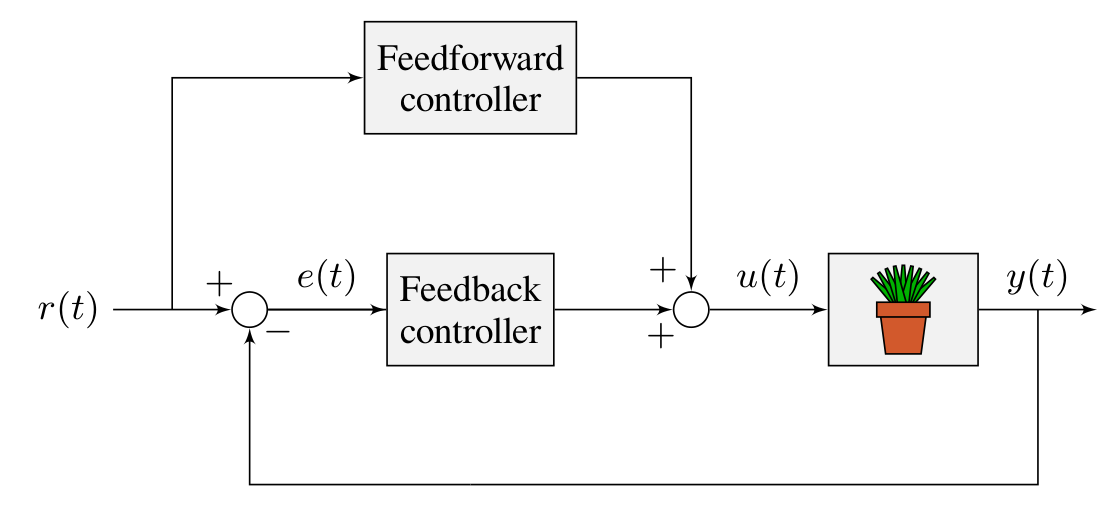
\includegraphics[width=0.85\textwidth]{fig1-6.png}
  \caption{同时具有前馈与反馈的控制系统}
  \label{fig:fffb}
\end{figure}

\section{前馈}
\label{sec:feedforward}
反馈控制对于参考值跟踪（让系统输出跟随期望的参考信号）可以很有效，但它是一种被动应对的措施——系统要等到已经落后于参考值之后，才会开始施加控制作用。如果我们能\textbf{提前}告诉控制器期望的运动和所需的输入，系统就能更快地响应，反馈控制器要做的功课也会更少。像这样把信息向前馈入被控对象的控制器称为前馈控制器（feedforward controller）。

前馈控制器注入的是关于系统动态的信息（就像模型所做的那样）或者关于期望运动的信息。前馈负责处理控制动作中我们已经知道的部分——即让系统跟踪参考值所必须施加的部分——而反馈则补偿我们在运行时不了解或无法了解的系统行为。

前馈有两类：基于模型的前馈（model-based feedforward）和针对未建模动态的前馈（feedforward for unmodeled dynamics）。前者求解系统的数学模型，得到满足期望速度和加速度所需的输入；后者直接补偿未建模的力或行为，让反馈控制器不必亲自处理它们。这两类前馈都能让反馈控制器变得更简单。我们将在后面的章节中给出这两类前馈的例子。

\section{为什么需要反馈控制？}
\label{sec:whyfeedback}
假设我们正在控制一台直流电机。只要拥有数学模型以及系统所有当前状态（即角速度）的知识，给定未来的电压输入，我们就能预测出所有未来的状态。既然如此，为什么还需要反馈控制？这是因为，如果系统受到任何未被我们的方程所建模的扰动——比如电枢上被施加了负载，或者电路其余部分的电压跌落导致指令电压与实际施加的电压不符——电机的角速度就会随时间偏离模型。

为了解决这个问题，我们可以对系统和环境进行测量，检测这种偏差并对它加以补偿。例如，我们可以测量当前的位置，并从中估计出角速度；然后，我们既向电机发出纠正指令，又把我们的模型拉回到与现实相符。这种反馈让我们能够应对不确定性，并对不确定性保持鲁棒。

\chapterphoto{UCSC McHenry 图书馆与 Media Theater 之间的小径}{photo-chap2}
\chapter{PID 控制器}

PID 控制器是一种常用的反馈控制器，由比例（proportional）、积分（integral）、微分（derivative）三项组成，PID 因此得名。本章将逐项构建 PID 控制器的定义，同时尽力为每一项的行为建立直觉。

首先，我们约定一些 PID 控制器的术语。参考值在这里称为设定值（setpoint，即期望位置），输出称为过程变量（process variable，即测量到的位置）。下面是相关量的一些常见变量命名约定：

\begin{center}
\begin{tabular}{ll}
  $r(t)$ & 设定值 \\
  $u(t)$ & 控制输入 \\
  $e(t)$ & 误差 \\
  $y(t)$ & 输出 \\
\end{tabular}
\end{center}

其中误差 $e(t) = r(t) - y(t)$。

对于已经熟悉 PID 控制的读者需要说明的是：本书的解读与经典的``过去、现在、未来''误差直觉并不一致。我们将从现代控制理论的视角出发，把比例控制器应用于我们所关心的不同物理量。这样能够更完整地解释导数项在设定值恒定和变化时的行为，而且这种直觉也会自然延续到本书后面介绍的现代控制方法中。

概括地说：比例项将\textbf{位置}误差驱动到零，微分项将\textbf{速度}误差驱动到零，而积分项随时间累积设定值曲线与输出曲线之间的面积（即位置误差的积分），并把当前的累积值加到控制输入上。下面我们对每一项展开详细讨论。

\section{比例项}
\label{sec:ptermm}

比例项将位置误差驱动到零。

\begin{definition}[比例控制器]
\begin{equation}
  u(t) = K_p e(t)
\end{equation}
其中 $K_p$ 是比例增益，$e(t)$ 是当前时刻 $t$ 的误差。
\end{definition}

图~\ref{fig:pblock} 展示了由 P 控制器控制的系统的框图。

\begin{figure}[htbp]
  \centering
  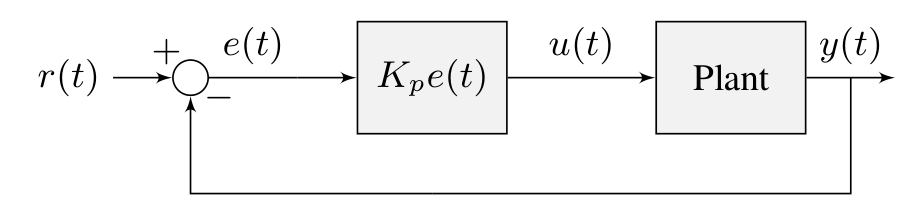
\includegraphics[width=0.85\textwidth]{fig2-1.png}
  \caption{P 控制器框图}
  \label{fig:pblock}
\end{figure}

比例增益的行为就像``用软件定义的弹簧''，把系统拉向期望的位置。回想物理课上学过的弹簧模型 $F = -kx$，其中 $F$ 是施加的力，$k$ 是比例常数，$x$ 是离开平衡点的位移。这个式子也可以写成 $F = k(0 - x)$，其中 $0$ 是平衡点。如果让平衡点成为反馈控制器的设定值，那么两个方程便一一对应：

\begin{align*}
  F &= k(r - x) \\
  u(t) &= K_p e(t) = K_p \left( r(t) - y(t) \right)
\end{align*}

也就是说，比例控制器把系统输出拉向设定值的``力''与误差成正比——正如弹簧一样。

\section{微分项}
\label{sec:dterm}

微分项将速度误差驱动到零。

\begin{definition}[PD 控制器]
\begin{equation}
  u(t) = K_p e(t) + K_d \frac{de}{dt}
\end{equation}
其中 $K_p$ 是比例增益，$K_d$ 是微分增益，$e(t)$ 是当前时刻 $t$ 的误差。
\end{definition}

图~\ref{fig:pdblock} 展示了由 PD 控制器控制的系统的框图。

\begin{figure}[htbp]
  \centering
  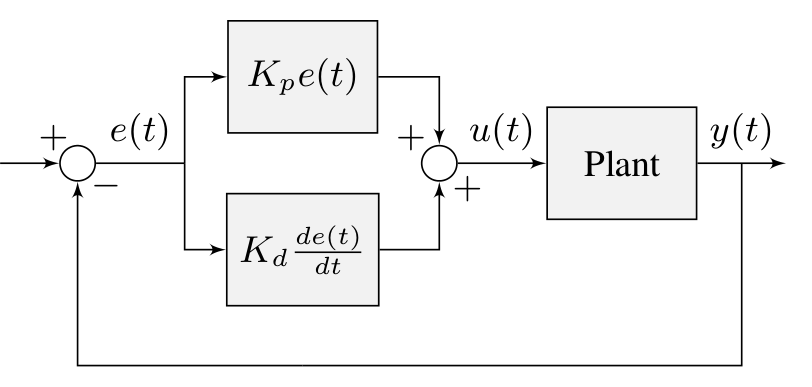
\includegraphics[width=0.9\textwidth]{fig2-2.png}
  \caption{PD 控制器框图}
  \label{fig:pdblock}
\end{figure}

PD 控制器包含一个位置比例控制器（$K_p$）和一个速度比例控制器（$K_d$）。速度设定值是由位置设定值随时间的变化隐式给出的。图~\ref{fig:pdelevator} 展示了电梯机构上的一个例子。

为了证明 PD 控制器其实就是两个比例控制器，我们对 PD 控制器的方程进行变形。设
\[
  u_k = K_p e_k + K_d \frac{e_k - e_{k-1}}{\Delta t}
\]
其中 $u_k$ 是第 $k$ 个时间步的控制输入，$e_k$ 是第 $k$ 个时间步的误差，$\Delta t$ 是时间步长。$e_k$ 定义为 $e_k = r_k - y_k$，其中 $r_k$ 是第 $k$ 个时间步的设定值，$y_k$ 是第 $k$ 个时间步的输出。

\begin{align*}
  u_k &= K_p (r_k - y_k) + K_d \frac{(r_k - y_k) - (r_{k-1} - y_{k-1})}{\Delta t} \\
  u_k &= K_p (r_k - y_k) + K_d \frac{r_k - y_k - r_{k-1} + y_{k-1}}{\Delta t} \\
  u_k &= K_p (r_k - y_k) + K_d \frac{r_k - r_{k-1} - y_k + y_{k-1}}{\Delta t} \\
  u_k &= K_p (r_k - y_k) + K_d \frac{(r_k - r_{k-1}) - (y_k - y_{k-1})}{\Delta t} \\
  u_k &= K_p (r_k - y_k) + K_d \left( \frac{r_k - r_{k-1}}{\Delta t} - \frac{y_k - y_{k-1}}{\Delta t} \right)
\end{align*}

注意，$\frac{r_k - r_{k-1}}{\Delta t}$ 是设定值的速度，$\frac{y_k - y_{k-1}}{\Delta t}$ 是系统速度的估计值。这意味着 PD 控制器的 $K_d$ 项把估计速度驱动到设定值速度。

如果设定值是恒定的，隐含的速度设定值就是零，因此当系统在运动时，$K_d$ 项会使它减速。它的作用就像``用软件定义的阻尼器''。这类阻尼器常见于闭门器上，其阻尼力随速度线性增大。

\begin{figure}[htbp]
  \centering
  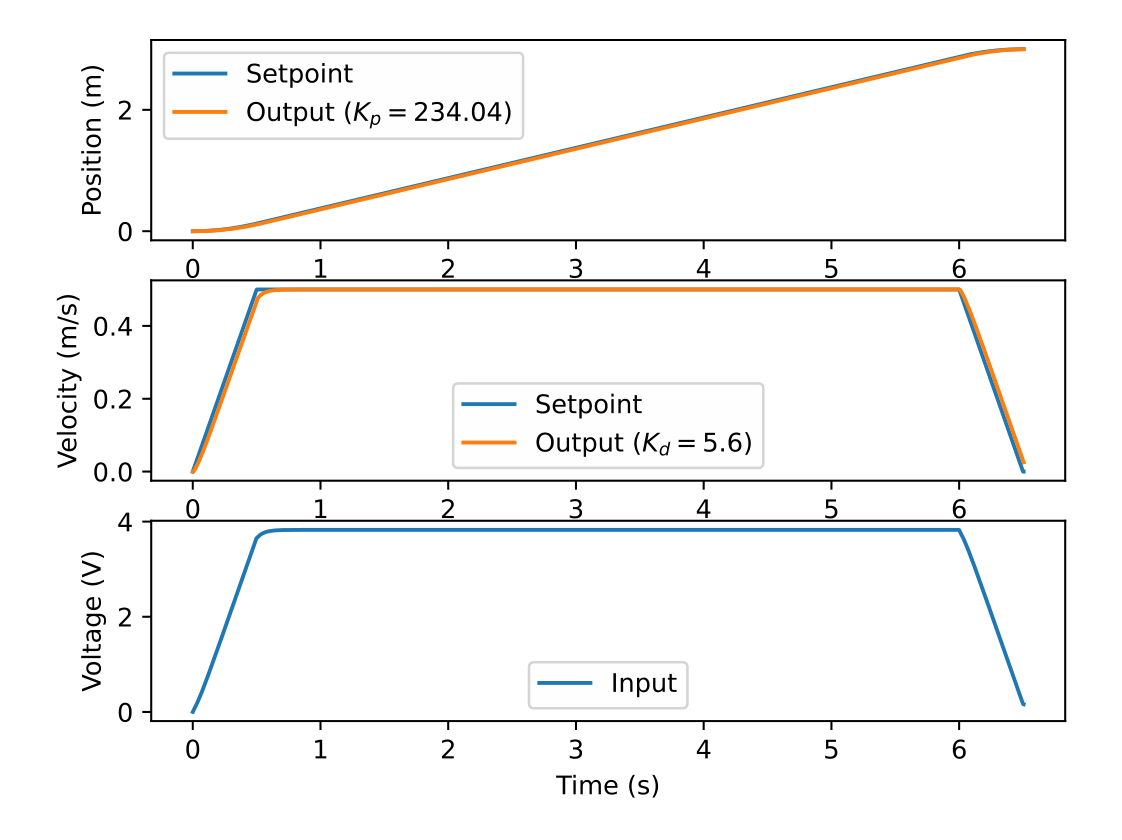
\includegraphics[width=0.62\textwidth]{fig2-3.png}
  \caption{电梯机构上的 PD 控制器}
  \label{fig:pdelevator}
\end{figure}

\section{积分项}
\label{sec:iterm}

积分项随时间累积设定值曲线与输出曲线之间的面积（即位置误差的积分），并把当前的累积值加到控制输入上。累积两条曲线之间的面积称为积分。

\begin{definition}[PI 控制器]
\begin{equation}
  u(t) = K_p e(t) + K_i \int_0^t e(\tau) \, d\tau
\end{equation}
其中 $K_p$ 是比例增益，$K_i$ 是积分增益，$e(t)$ 是当前时刻 $t$ 的误差，$\tau$ 是积分变量。
\end{definition}

积分从时刻 $0$ 一直积到当前时刻 $t$。我们用 $\tau$ 表示积分变量，因为在积分过程中需要一个能够取多个值的变量，而 $t$ 已经被定义为当前时间，不能再使用。

图~\ref{fig:piblock} 展示了由 PI 控制器控制的系统的框图。

\begin{figure}[htbp]
  \centering
  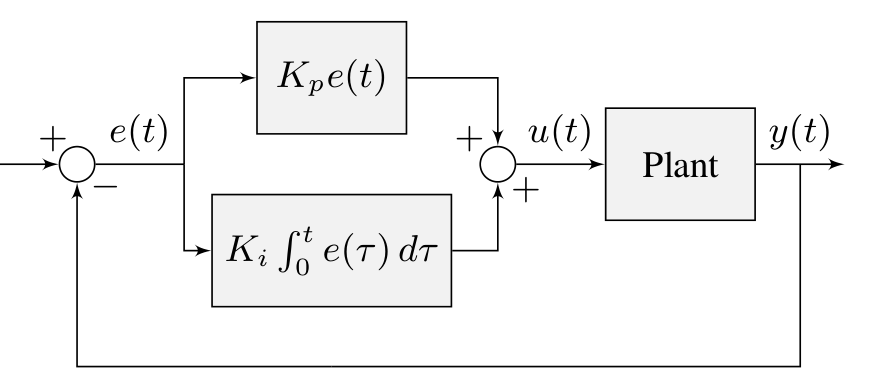
\includegraphics[width=0.9\textwidth]{fig2-4.png}
  \caption{PI 控制器框图}
  \label{fig:piblock}
\end{figure}

当系统在稳态下已经非常接近设定值时，比例项可能太小，不足以把输出一路拉到设定值，而此时微分项为零。这就可能造成稳态误差，如图~\ref{fig:sse} 所示。

消除稳态误差的一种常用方法是对误差进行积分，并将其加到控制输入上。这会使控制量不断增大，直到系统收敛为止。图~\ref{fig:sse} 展示了飞轮出现稳态误差的例子；图~\ref{fig:pi-nosse} 展示了在飞轮控制器中加入积分器之后如何消除了稳态误差。然而，积分增益过大会导致超调，如图~\ref{fig:pi-overshoot} 所示。

\begin{tip}
消除稳态误差还有更好的办法，例如使用前馈，或者利用对系统的其他知识来约束积分控制作用的时机。我们讲到现代控制理论时会更详细地讨论这些内容。
\end{tip}

\begin{figure}[htbp]
  \centering
  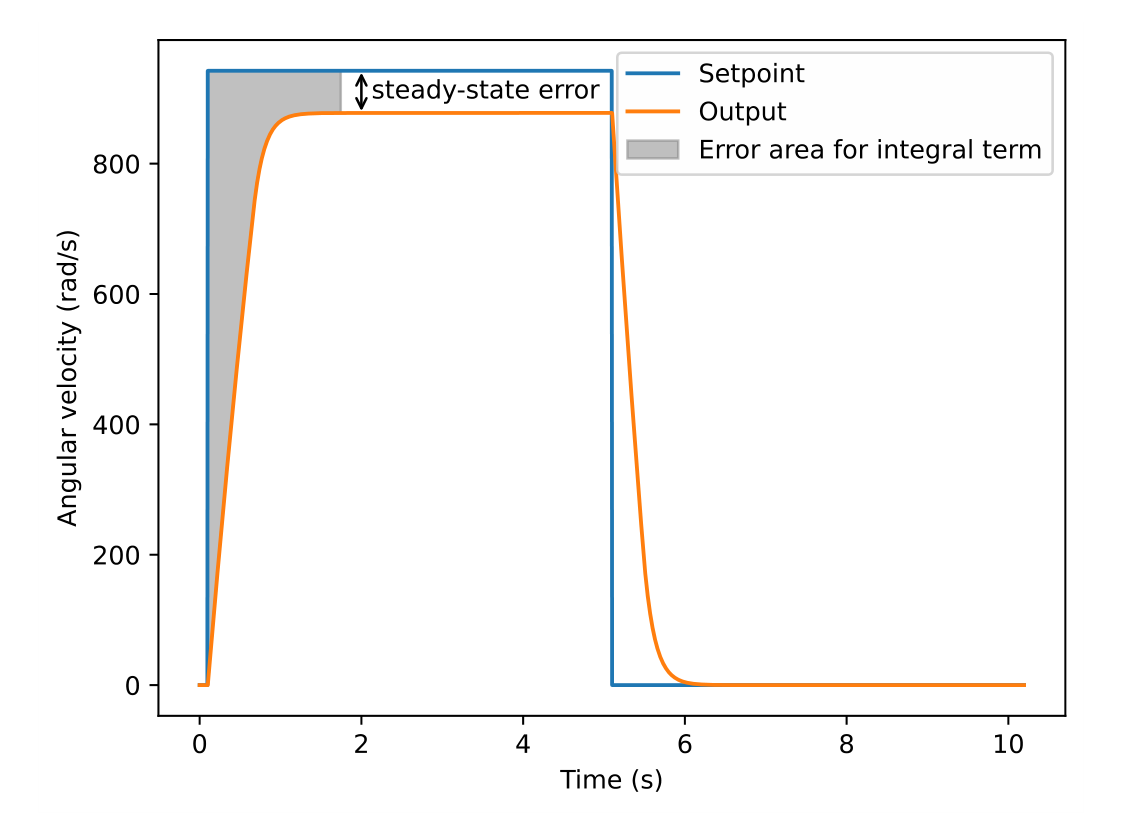
\includegraphics[width=0.62\textwidth]{fig2-5.png}
  \caption{飞轮上带有稳态误差的 P 控制器}
  \label{fig:sse}
\end{figure}

\begin{figure}[htbp]
  \begin{minipage}[t]{0.48\textwidth}
    \centering
    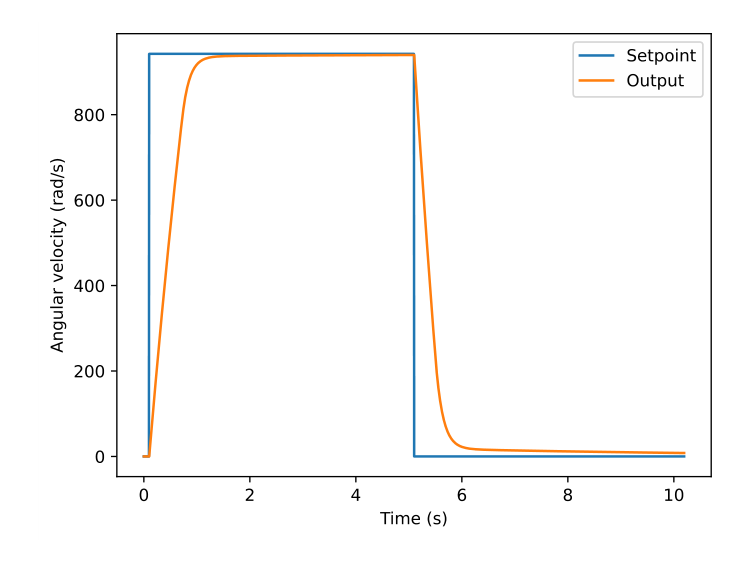
\includegraphics[width=\linewidth]{fig2-6.png}
    \caption{飞轮上无稳态误差的 PI 控制器}
    \label{fig:pi-nosse}
  \end{minipage}\hfill
  \begin{minipage}[t]{0.48\textwidth}
    \centering
    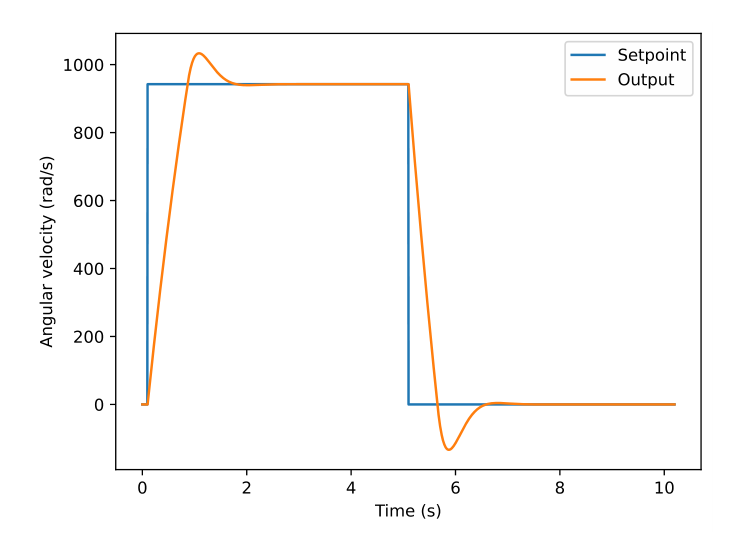
\includegraphics[width=\linewidth]{fig2-7.png}
    \caption{$K_i$ 增益过大导致超调的飞轮 PI 控制器}
    \label{fig:pi-overshoot}
  \end{minipage}
\end{figure}

\section{PID 控制器的定义}
\label{sec:piddef}

把这三项组合起来，就得到了 PID 控制器的典型定义。

\begin{definition}[PID 控制器]
\begin{equation}
  u(t) = K_p e(t) + K_i \int_0^t e(\tau) \, d\tau + K_d \frac{de}{dt}
\end{equation}
其中 $K_p$ 是比例增益，$K_i$ 是积分增益，$K_d$ 是微分增益，$e(t)$ 是当前时刻 $t$ 的误差，$\tau$ 是积分变量。
\end{definition}

图~\ref{fig:pidblock} 展示了由 PID 控制器控制的系统的框图。

\begin{figure}[htbp]
  \centering
  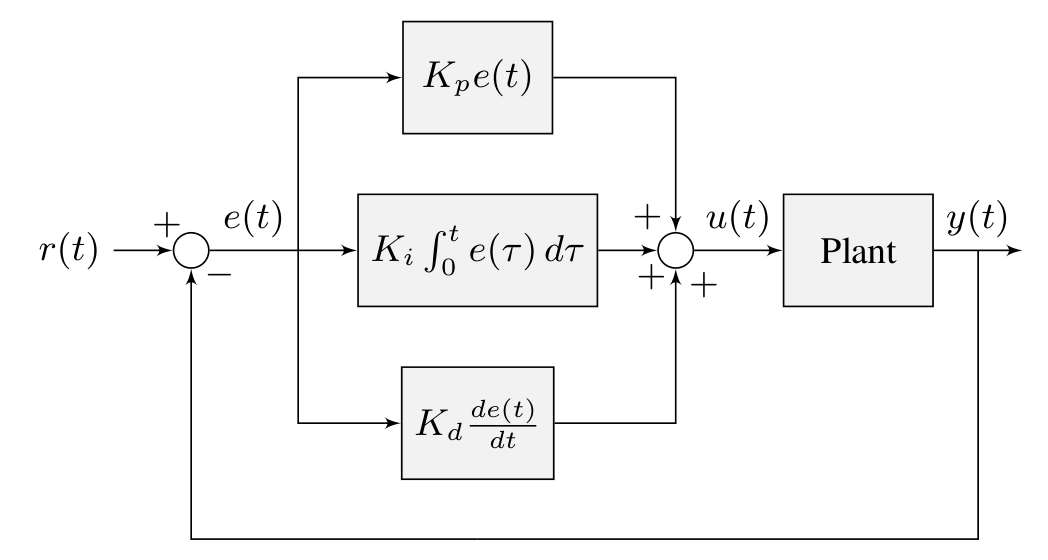
\includegraphics[width=0.9\textwidth]{fig2-8.png}
  \caption{PID 控制器框图}
  \label{fig:pidblock}
\end{figure}

\section{响应类型}
\label{sec:responsetypes}

由 PID 控制器驱动的系统一般有三种响应类型：欠阻尼、过阻尼和临界阻尼。如图~\ref{fig:responses} 所示。

\begin{figure}[htbp]
  \centering
  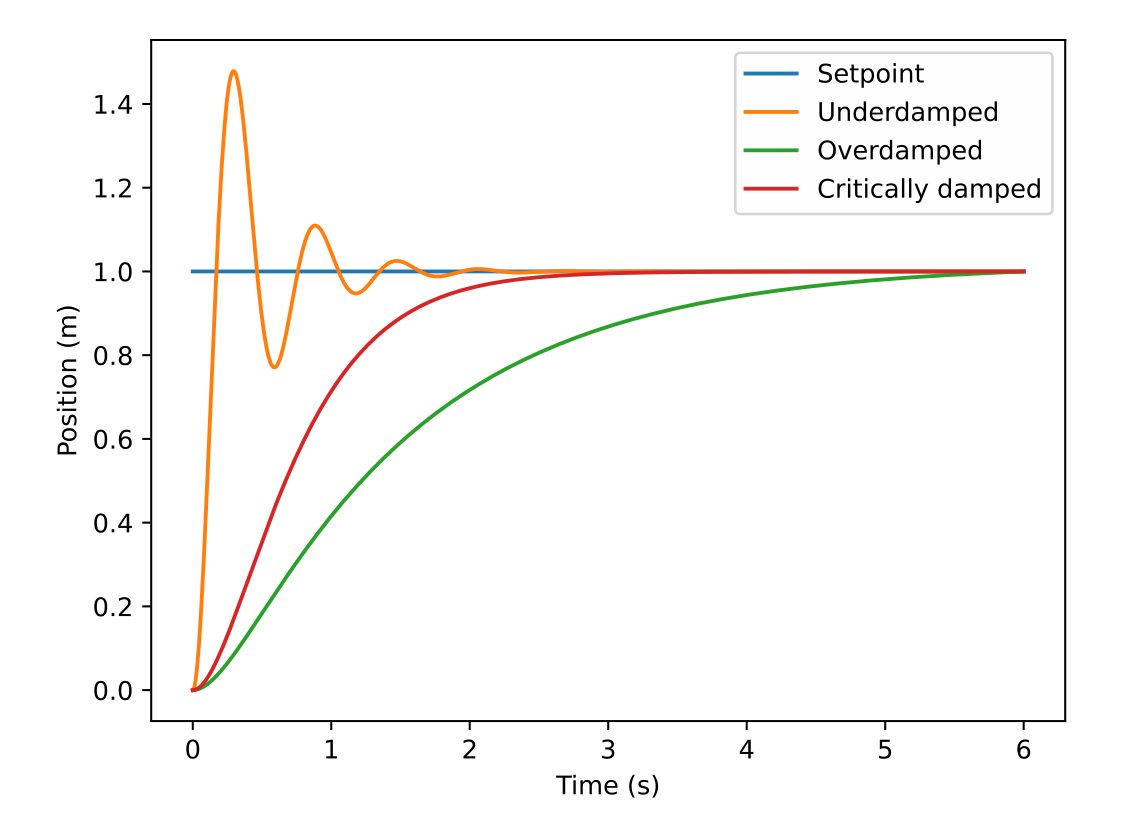
\includegraphics[width=0.62\textwidth]{fig2-9.png}
  \caption{PID 控制器的响应类型}
  \label{fig:responses}
\end{figure}

对于图~\ref{fig:responses} 中的阶跃响应：上升时间（rise time）是系统在施加阶跃输入后首次到达参考值所花的时间；调节时间（settling time）是系统在施加阶跃输入后在参考值处稳定下来所花的时间。

欠阻尼响应在稳定之前会围绕参考值振荡。过阻尼响应上升缓慢，且不会越过参考值。临界阻尼响应在不围绕参考值振荡（即先过冲后回落）的前提下，具有最短的上升时间。

\section{手动整定}
\label{sec:manualtuning}

以下步骤适用于位置式 PID 控制器。速度式 PID 控制器通常不需要 $K_d$。

\begin{enumerate}
  \item 将 $K_p$、$K_i$ 和 $K_d$ 置零。
  \item 增大 $K_p$，直到输出开始在设定值附近振荡。
  \item 在不引起系统响应抖动的前提下，尽可能增大 $K_d$。
\end{enumerate}

如果设定值遵循梯形曲线（见第 15.1 节），整定会容易得多。将位置设定值、速度设定值、测量位置和测量速度都绘制出来。速度设定值可以通过对位置设定值做数值微分得到（即 $v_{\text{desired},k} = \frac{r_k - r_{k-1}}{\Delta t}$）。先增大 $K_p$，直到位置跟踪良好；然后增大 $K_d$，直到速度跟踪良好。

如果控制器最终稳定在高于或低于设定值的输出上，可以增大 $K_i$，使控制器在合理的时间内到达设定值。

\begin{tip}
如果有模型可用（基于输出的控制并非如此），应优先使用前馈（第 7.8 节）或在被控对象中引入积分器（第 6.7 节），而不是在控制器中使用积分器（例如 PID 的 I 项）。积分器只应用于补偿无法建模的动态。
\end{tip}

注意，如果 $K_i$ 过大，就可能发生积分饱和（integral windup）：设定值发生大幅变化后，积分项累积的误差可能超过最大控制输入。结果，系统会超调并持续增大，直到这部分累积的误差被释放为止。

\section{局限性}
\label{sec:limitations}

当对系统动态没有任何先验知识时，PID 的启发式整定方法是合理的选择。然而，如果已知系统的动力学模型，就可以设计出响应好得多的控制器。此外，PID 只适用于单输入单输出（SISO）系统；我们将在本书第二部分介绍多输入多输出（MIMO）系统的控制方法。

\chapterphoto{UCSC Crown/Merrill 公交站旁的林线}{photo-chap3}
\chapter{应用建议}

\section{机械方案与软件方案}
\label{sec:mechvssw}

虽然本书聚焦于控制工程在 FRC 中的应用，但要打造一支成功的队伍，控制并非必需；FRC 主要是一项机械竞赛，而不是软件竞赛。我们花费六个多星期来设计和建造机器人，却常常只给软件测试留出两天时间。尽管如此，各队伍依然能派出有竞争力的机器人——这也证明了如今 FRC 软件生态是多么简单易用。首先应当专注于可靠的机械设计，因为好的机械设计配上简单的软件就能成功，而不可靠的硬件则无论如何都无法让机器人成功。

一个设计问题的解决方案，可能是机械复杂度与软件复杂度之间的权衡。例如，对于一个只需要两个位置的机构，与``电机 + 旋转编码器 + 软件反馈控制''相比，一个连接到气动执行器的电磁阀可能更省事、也更可靠。不过，如果软件方案能够顺利实现，机器人就可以省去空气压缩机和储气罐所占的空间和重量。

我评估设计的经验法则是：优先选择优雅的机械方案，而不是面面俱到的软件方案，因为在比赛中让机械方案变得可靠要更容易。布置合理的传感器也能大幅提升机器人的表现，并减轻操作手的认知负担。例如在 2011 年 FRC 比赛中，用一个限位开关加比赛计时器，就能在终局（endgame）开始时自动释放 minibots。许多情况下，手动流程可以之后再自动化，并且在相关软件或传感器失效时保留手动后备方案。对于必须依赖闭环控制才能工作的设计要保持谨慎。

什么样的问题应当用硬件而不是用巧妙的控制软件来解决？控制可以应对诸如电池电压跌落或测量噪声之类的扰动，但它的能力是有限度的。例如，面对底盘变速箱卡死或者掉链条，软件是无能为力的。有时候，直接在硬件上修好问题的根源才是更好的选择。

设计机器人机构时要考虑可控性（controllability）。FRC 971 队的``Mechanical Design for Controllability''研讨会对这个问题有更详细的论述。从中总结出的两个要点是：

\begin{itemize}
  \item 减小齿轮箱的回差（backlash）
  \item 选择能够提供足够控制能力的电机和减速比
\end{itemize}

\begin{media}[视频资源]
``Spartan Series / Mechanical Design for Controllability''（时长 1 小时 31 分钟）\\
Travis Schuh\\
\url{https://youtu.be/VNfFn-gcfFI}
\end{media}

请记住，``用软件修补''并不总是答案。本书剩余的章节假设你已经完成了工程分析，并得出结论：你所选的设计会从更复杂的控制中获益，而且你有时间或有专长把它实现出来。

\section{执行器饱和}
\label{sec:saturation}

反馈控制器根据参考值与当前状态之间的误差来计算输出。现实世界中的被控对象，其可供反馈控制器使用的控制能力并不是无限的。当达到执行器的限制时，反馈控制器的表现就好像增益被暂时降低了（也就是说，它的控制能力下降了）。

我们用一点数学来解释这一点。设控制器为 $u = k(r - x)$，其中 $u$ 是控制量，$k$ 是增益，$r$ 是参考值，$x$ 是当前状态。令 $u_{\max}$ 为执行器输出的上限（它小于 $u$ 未封顶时的取值），$k_{\max}$ 为与之对应的最大增益。现在针对相同的参考值和当前状态，比较封顶与未封顶的控制器：

\begin{align*}
  u_{\max} &< u \\
  k_{\max} (r - x) &< k (r - x) \\
  k_{\max} &< k
\end{align*}

要使不等式成立，$k_{\max}$ 必须小于原来的 $k$。当系统响应中状态随时间呈线性变化、而不是在接近参考值时呈指数变化，就能明显看出这种增益的降低。这是因为此时控制量不再遵循衰减指数曲线。一旦系统更接近参考值，控制器就会停止饱和，重新给出符合实际的控制器输出。

\chapterphoto{圣玛丽亚与文图拉之间北行高速公路旁的山丘}{photo-chap4}
\chapter{微积分}

本书会偶尔使用导数和积分：前者表示量在时间上的微小变化，后者表示量随时间的无穷小累加。这里给出的公式和表格，足以支撑你在后续章节中完成数学推导。

如果你读完后想了解更多，3Blue1Brown 的《Essence of calculus》系列对这些概念的介绍非常精彩。

\begin{media}[视频资源]
``Essence of calculus''（微积分的本质）\\
3Blue1Brown\\
\url{https://www.3blue1brown.com/?topic=calculus}
\end{media}

\section{导数}
\label{sec:derivatives}

导数（derivative）是表示曲线在任意点处斜率的表达式。对形如 $f(x)$ 的函数施行这一运算的常用记号包括：

\begin{table}[htbp]
  \centering
  \begin{tabular}{lll}
    \toprule
    莱布尼茨记号 & 拉格朗日记号 & 牛顿记号 \\
    \midrule
    $\dfrac{d}{dx} f(x)$  & $f'(x)$    & $\dot{f}(x)$ \\
    $\dfrac{d^2}{dx^2} f(x)$ & $f''(x)$ & $\ddot{f}(x)$ \\
    $\dfrac{d^3}{dx^3} f(x)$ & $f'''(x)$ & $\dottriple{f}(x)$ \\
    $\dfrac{d^4}{dx^4} f(x)$ & $f^{(4)}(x)$ & $\dotquad{f}(x)$ \\
    $\dfrac{d^n}{dx^n} f(x)$ & $f^{(n)}(x)$ & $\overset{n}{\dot{f}}(x)$ \\
    \bottomrule
  \end{tabular}
  \caption{$f(x)$ 的导数记号}
  \label{tab:deriv-notation}
\end{table}

拉格朗日记号读作``f 一撇''（f prime of x）、``f 两撇''（f double-prime of x）等。牛顿记号读作``f 加一点''（f dot of x）、``f 加两点''（f double-dot of x）等。

\subsection{幂法则}
\label{sec:powerrule}

\begin{align*}
  f(x) &= x^n \\
  f'(x) &= n x^{n-1}
\end{align*}

\subsection{乘积法则}
\label{sec:productrule}

乘积法则用于对两个表达式的乘积求导。

\begin{align*}
  h(x) &= f(x) \, g(x) \\
  h'(x) &= f'(x) \, g(x) + f(x) \, g'(x)
\end{align*}

\subsection{链式法则}
\label{sec:chainrule}

链式法则用于对嵌套的表达式求导。

\begin{align*}
  h(x) &= f(g(x)) \\
  h'(x) &= f'(g(x)) \cdot g'(x)
\end{align*}

例如：

\begin{align*}
  h(x) &= (3x + 2)^5 \\
  h'(x) &= 5 \, (3x + 2)^4 \cdot (3) \\
  h'(x) &= 15 \, (3x + 2)^4
\end{align*}

\subsection{偏导数}
\label{sec:partialderivatives}

多元函数的偏导数（partial derivative）是该函数对其中某一个变量求导，而其余变量保持不变（这与全导数不同，全导数允许所有变量同时变化）。在莱布尼茨记号中，偏导数用 $\partial$ 代替 $d$。

例如，设 $h(x, y) = 3xy + 2x$。求对 $x$ 的偏导数时，把 $y$ 当作常数：

\[
  \frac{\partial h(x,y)}{\partial x} = 3y + 2
\]

求对 $y$ 的偏导数时，$x$ 被当作常数，因此第二项变为零：

\[
  \frac{\partial h(x,y)}{\partial y} = 3x
\]

\section{积分}
\label{sec:integrals}

积分（integral）是导数的逆运算，用于计算曲线下的面积。下面基于表~\ref{tab:common-deriv-int} 给出一个例子：

\[
  \int e^{at} \, dt = \frac{1}{a} e^{at} + C
\]

需要引入任意常数 $C$，是因为求导时常数会被丢弃——竖直方向的平移不影响斜率。在做逆运算时，我们没有足够的信息来确定这个常数。

不过，我们可以为积分加上积分限：

\begin{align*}
  \int_0^t e^{at} \, dt
    &= \left. \left( \frac{1}{a} e^{at} + C \right) \right|_0^t \\
    &= \left( \frac{1}{a} e^{at} + C \right) - \left( \frac{1}{a} e^{a \cdot 0} + C \right) \\
    &= \left( \frac{1}{a} e^{at} + C \right) - \left( \frac{1}{a} + C \right) \\
    &= \frac{1}{a} e^{at} + C - \frac{1}{a} - C \\
    &= \frac{1}{a} e^{at} - \frac{1}{a}
\end{align*}

这样做之后，任意常数就抵消了。

\section{变量代换}
\label{sec:changeofvariables}

变量代换（change of variables）是一种简化问题的技巧：把表达式替换成新的变量，使问题变得更易处理。这既可以意味着问题变得更直接，也可以意味着问题化成了某种已有成熟求解工具的常见形式。下面是一个利用变量代换求积分的例子：

\[
  \int \cos \omega t \, dt
\]

令 $u = \omega t$，则

\begin{align*}
  du &= \omega \, dt \\
  dt &= \frac{1}{\omega} \, du
\end{align*}

现在把 $u$ 和 $dt$ 的表达式代入：

\begin{align*}
  \int \cos u \, \frac{1}{\omega} \, du
    &= \frac{1}{\omega} \int \cos u \, du \\
    &= \frac{1}{\omega} \sin u + C \\
    &= \frac{1}{\omega} \sin \omega t + C
\end{align*}

另一个例子——当我们真正讲到状态空间记号（$\dot{x} = Ax + Bu$）时会用到——是闭环状态空间系统：

\begin{align*}
  \dot{x} &= (A - BK)x + BKr \\
  \dot{x} &= A_{\mathrm{cl}} x + B_{\mathrm{cl}} u_{\mathrm{cl}}
\end{align*}

其中 $A_{\mathrm{cl}} = A - BK$，$B_{\mathrm{cl}} = BK$，$u_{\mathrm{cl}} = r$。由于它与开环系统的形式一致，所有相同的分析工具都可以直接用于它。

\section{常用表}
\label{sec:tables}

\subsection{常用导数与积分}
\label{sec:commonderivatives}

\begin{table}[htbp]
  \centering
  \begin{tabular}{lll}
    \toprule
    $\displaystyle\int f(x) \, dx$ & $f(x)$ & $f'(x)$ \\
    \midrule
    $ax$ & $a$ & $0$ \\
    $\dfrac{1}{2} a x^2$ & $ax$ & $a$ \\
    $\dfrac{1}{a+1} x^{a+1}$ & $x^a$ & $a x^{a-1}$ \\
    $\dfrac{1}{a} e^{ax}$ & $e^{ax}$ & $a e^{ax}$ \\
    $-\cos(x)$ & $\sin(x)$ & $\cos(x)$ \\
    $\sin(x)$ & $\cos(x)$ & $-\sin(x)$ \\
    $\cos(x)$ & $-\sin(x)$ & $-\cos(x)$ \\
    $-\sin(x)$ & $-\cos(x)$ & $\sin(x)$ \\
    \bottomrule
  \end{tabular}
  \caption{常用导数与积分}
  \label{tab:common-deriv-int}
\end{table}

\section{微分方程}
\label{sec:odes}

微分方程（differential equation）是含有导数的方程。

设 $y$ 是 $x$ 的未知函数，$f$ 是给定的 $x$ 的函数。\textbf{常微分方程}（ODE）包含一个单变量 $x$ 的未知函数、该未知函数的导数，以及 $x$ 的给定函数。例如：

\[
  \frac{dy}{dx} = f(x)
\]

设 $y$ 是 $x_1$ 和 $x_2$ 的未知函数。\textbf{偏微分方程}（PDE）包含未知的多元函数及其偏导数。例如：

\[
  y(x_1, x_2) = x_1 \frac{\partial y}{\partial x_1} + x_2 \frac{\partial y}{\partial x_2}
\]

某些 ODE 和 PDE 有闭式解（例如 ODE $\frac{dy}{dx} = ay$ 的解为 $y(x) = y(0) e^{ax}$），但大多数方程必须用计算机进行数值求解。


\backmatter
\end{document}
